\label{sec: symmetries}
For any initial condition $p_0 = (c_0, R_0) \in \mathcal{P}$ and any control curve $\xi: I \subseteq \R \to \M$, with $I$ a neighborhood of zero, we denote by $\gamma(c_0, R_0, \xi): I \to \mathcal{P}$ the solution associated to the dynamical system
\begin{equation}
\label{eq:dynamical system}
\begin{aligned}
	&\dot{p} = F(R, \xi) \dot{\xi},& & p(0) := p_0,
\end{aligned}
\end{equation}
as well as $\gamma_c(c_0, R_0, \xi)$ and $\gamma_\theta(c_0, R_0, \xi)$ its projections on $\R^3$ and $\SO(3)$, respectively, such that for any $t \in I$
\begin{equation}
	\dot{\gamma}(c_0, R_0, \xi)(t) = F(\gamma_\theta(c_0, R_0, \xi)(t), \xi(t))\dot{\xi}(t).
\end{equation}

\subsection{Rotational invariance}
Rotational invariance of the Stokes equations expresses the fact that solution of the dynamical system (\ref{eq:dynamical system}) is invariant under rotations, i.e., that for any rotation $R \in \SO(3)$ we have for the spatial part of the solution
\begin{equation}
\label{eq:spatial rotational invariance}
	\gamma_c(c_0, R R_0, \xi)(t) = R \gamma_c (c_0, R_0, \xi)(t) + (I - R) c_0
\end{equation}
and for the angular part of the solution
\begin{equation}
\label{eq: angular rotational invariance}
	\gamma_\theta(c_0, R R_0, \xi)(t) =  R \gamma_\theta(c_0, R_0, \xi)(t)
\end{equation}
at any point in time $t \in I$. Eventually, we can rigorously state the following symmetry property of the control system (\ref{eq:dynamical system}) with respect to rotations:

\begin{condition}[Rotational invariance]
\label{cond:rotational invariance}
If $\gamma(c_0, R_0, \xi)$ is a solution of the control system (\ref{eq:dynamical system}), then so is $\gamma(c_0, R R_0, \xi)$ and (\ref{eq:spatial rotational invariance}) and (\ref{eq: angular rotational invariance}) hold.
\end{condition}

\begin{remark}
To follow the reasoning of \cite{Alouges2017}, the symmetry relations satisfied by \textsc{SPr4} are stated as hypotheses on the solution $\gamma$. In so doing, the results work for any control system of the form (\ref{eq: control system}) and satisfying the hypotheses we state, e.g. rotational invariance, independently of these hypotheses being guaranteed by the invariance of the Stokes equations under a certain group of transformations. 
\end{remark}
We then have
\begin{proposition}
\label{prop: rotational invariance}
Let $\xi_0 := \xi(0) \in \M$ denote the initial state of the control parameters and by $T_{\xi}\M$ the tangent space of $\M$ at $\xi$. If the control system (\ref{eq:dynamical system}) is invariant under rotations and for every $\xi \in \M$ it holds that $T_{\xi} \M \simeq \R^4$, then
\begin{equation}
	F_c(R, \xi) = R F_c(\xi) \text { and } F_\theta(R, \xi) = R F_{\theta} (R, \xi),
\end{equation}
for every $(R, \xi) \in \SO(3) \times \M$, where $F_c(\xi) := F_{c}(I, \xi)$ and $F_{\theta}(\xi) := F_{\theta}(I, \xi)$. 
\end{proposition}

\begin{proof}
On the one hand, we have by definition of the dynamical system (\ref{eq: control system}) that
\begin{equation}
	\dot{\gamma}_c(c_0, R, \xi) = F_c(\gamma_{\theta}(c_0, R, \xi), \xi) \dot{\xi}.
\end{equation}
On the other hand, using equation (\ref{eq:spatial rotational invariance}) and once more the definition of the dynamical system (\ref{eq:dynamical system}), we obtain
\begin{equation}
	\dot{\gamma}_c (c_0, R, \xi) = R  \dot{\gamma}_c(c_0, I, \xi) = 
	R F_c(\gamma_{\theta}(c_0, I, \xi), \xi) \dot{\xi}.
\end{equation}
Therefore, $F_c(\gamma_{\theta}(c_0, R, \xi), \xi) \dot{\xi} = R F_{c}(\gamma_{\theta}(c_0, I, \xi), \xi) \dot{\xi}$ for every $R \in \SO(3)$. Since $T_{\xi_0} \M \simeq \R^4$, evaluation of the preceding expression at $t = 0$ yields $F_{c}(R, \xi_0) = R F_{c}(I, \xi_0)$, as desired. The proof for $F_{\theta}$ is completely analogous and thus is omitted.
\end{proof}

\subsection{Permutation of two arms}
In this section, we investigate the effect of a swap of two arms on the generic solution of the dynamical system (\ref{eq:dynamical system}).
To that end, let $P_{ij} \in M_{4 \times 4}(\R)$ denote the permutation matrix that interchanges the $i$-th and $j$-th index of a vector, which corresponds to the swap of the arms $||i$ and $||j$, denoted by $(||i\leftrightsquigarrow ||j$), if applied to the shape space $\M$. In addition, let $S_{ij}$ denote the reflection of $\R^3$ sending arm $||i$ onto arm $||j$ in the reference orientation $I$. Geometrical inspection of the reference tetrahedron shows that $S_{ij}$ is always a reflection at a plane containing the remaining arms $||k$ and $||l$.

Before we formulate the symmetry conditions for the interchanging of two arms, we recall some results about how rotations behave under reflections. So far, we have only regarded the orientation of \textsc{SPr4} as a rotation matrix in $\SO(3)$. However, by Euler's rotation theorem to every such rotation matrix $R \in \SO(3)$ there exists a corresponding rotation vector $\omega \in \R^3$ which is collinear to the unique axis of rotation defined by $R$, i.e. $\omega$ is an eigenvector associated to the eigenvalue 1 of $R$. Its length is given by the angle of rotation around this axis. The rotation vector $\omega$ is then directly related to the rotation matrix $R$ via the map $\exp: \so(3) \to \SO(3)$, where $\so(3) = T_I \SO(3) = \Skew_3(\R)$ denotes the Lie algebra over $\SO(3)$, which we will illustrate in the following paragraphs.


It is clear that $\dim \Skew_3(\R) = 3$. In particular, if $R_1(\theta), R_2(\theta)$ and $R_3(\theta)$ denote the simple rotations around the $\hat{e}_1$-, $\hat{e}_2$- and $\hat{e}_3$-axis, where $\hat{e}_1, \hat{e}_2, \hat{e}_3$ denote the canonical basis vectors of $\R^3$, then the matrices
\begin{align}
\label{eq: L1}
	&L_1 = \frac{\dd}{\dd\theta}R_1(\theta)_{\mid \theta =0} = \left(\begin{array}{ccc}
	0 & 0 & 0 \\ 
	0 & 0 & -1 \\ 
	0 & 1 & 0
	\end{array}  \right ),\\
\label{eq: L2}
	&L_2 = \frac{\dd}{\dd\theta}R_2(\theta)_{\mid \theta =0} = \left (\begin{array}{ccc}
	0 & 0 & 1 \\ 
	0 & 0 & 0 \\ 
	-1 & 0 & 0
	\end{array}  \right ),\\
\label{eq: L3}
	&L_3 = \frac{\dd}{\dd\theta}R_3(\theta)_{\mid \theta =0} = \left (\begin{array}{ccc}
	0 & -1 & 0 \\ 
	1 & 0 & 0 \\ 
	0 & 0 & 0
	\end{array}  \right ),
\end{align}
form a basis of $\so(3)$, denoted by $\mathcal{L}$, consisting of the infinitesimal rotations around the corresponding axes. A trivial computation then shows that $R = \exp\left ( \sum_{k \in \N_3} \omega_k L_k \right )$. 
% If we now write $\textbf{L} := (L_1, L_2, L_3)^T$ and allow the slight abuse of notation
%\begin{align}
%	\omega \cdot \mathbf{L} = \omega_1 L_1 + \omega_2 L_2 + \omega_3 L_3,
%\end{align}
%we find by direct computation that $\exp(\omega \cdot \mathbf{L}) = R$. This relationship allows us to formulate the behavior of the orientation of \textsc{SPr4} under reflection and thus under permutation of two arms as we shall see later. Indeed, we have

%\begin{lemma}
%\label{lem:mirror image of orientation}
%For any orientation of a rigid body characterized by $R \in \SO(3)$, the orientation of its mirror image under a reflection $S$ is given by
%\begin{align}
%	\tilde{R} = S R S.
%\end{align}
%\end{lemma}
%
%\begin{proof}
%Let us first consider the simple case where $S_i$ is the reflection of the $\hat{e}_i$-axis. Let $\omega$ and $\tilde{\omega}$ be the rotation vectors corresponding to $R$ and $\tilde{R}$, respectively. They are related by $\tilde{\omega} = -S_i \omega$, where the gain of the minus sign stems from the fact that rotation vectors are in fact pseudovectors. In other words, we not only reflect the axis of rotation but we also reverse the sense of rotation around the axis. It follows then from direct computation that
%\begin{equation}
%\label{eq: transformation of rotation axis}
% \tilde{\omega} \cdot \mathbf{L} = (-S_i\omega) \cdot \mathbf{L} = S_i(\omega \cdot \mathbf{L})S_i
%\end{equation}
%and thus we have
%\begin{equation}
%\tilde{R} = \exp(\tilde{\omega} \cdot \mathbf{L}) = \exp(S_i(\omega \cdot \mathbf{L})S_i) = S_iRS_i,
%\end{equation}
%as $S_i^{-1} = S_i$.
%
%If now $S$ is an arbitrary reflection, we always find a rotation $Q \in \SO(3)$ such that $S = Q S_i Q^T$ for one of the elementary reflections $S_i$. Moreover, for any rotation $R' \in \SO(3)$ we find another $R \in \SO(3)$ such that $R' = Q R Q^T$. In particular, we have
%\begin{equation}
%\tilde{R}' = Q \tilde{R} Q^T = Q S_iRS_i Q^T = S R' S^T,
%\end{equation}
%as desired.
%\end{proof}
However, to clearly state the relations between reflections and orientations, let us first fix some notation. We denote by $\mathcal{E} := (e_1, e_2, e_3, e_4)$ the canonical basis for $\R^4$. Then we denote the matrix representing an arbitrary linear map $T: V \to W$ between two vector spaces $V$ and $W$ with respect to two bases $\mathcal{B}$ and $\mathcal{C}$ by $[T]_{\mathcal{B}}^{\mathcal{C}}$. Subsequently, we will especially make use of the adjoint map on $\so(3)$ associated to an orthogonal transformation $Q$ of $\R^3$. More precisely, if $Q$ is an orthogonal transformation of $\R^3$, we define the adjoint map $\ad_Q : \so(3) \to \so(3)$ by
\begin{equation}
\ad_Q(M) := Q M Q^T,
\end{equation}
which is clearly a linear map. Then we have the following result about orthogonal transformations and their adjoint maps, which we state in a rather general fashion as this will be beneficial at a later stage.

\begin{lemma}
\label{lem:mirror image of orientation}
Let $S, Q:\R^3 \to \R^3$ be a reflection at a plane and a rotation of $\R^3$, respectively. Then the representation matrices of their adjoint maps are given by
\begin{eqnarray}
[\ad_{S}]_{\mathcal{L}} = -S & \text{and}  & [\ad_{Q}]_{\mathcal{L}} = Q.
\end{eqnarray}
In particular, if $R \in \SO(3)$ characterizes the orientation of a rigid body, the orientation $\tilde{R}$ of its mirror image under a reflection $S$ is characterized by $\tilde{R} = SRS$.
\end{lemma}

\begin{proof}
Let us denote by $S_i$ the reflection of the $\hat{e}_i$ axis. Then one finds by a straightforward computation that the first statement is true for $S_i$ and $R_i(\theta)$ for all $\theta \in \R$ and $i \in \N_3$. Now the statement follows by decomposing any rotation $Q \in \SO(3)$ into its Euler angles and any reflection $S$ into $S = Q S_i Q^{T}$ for some rotation $Q$ and one of the elementary reflections $S_i$.

For the second part, let $S$ be an arbitrary reflection in $\R^3$ and let us denote by $\tilde{\omega}$ the rotation vector of the mirror image. Since the rotation vector of a rigid body is a pseudovector, we have $\tilde{\omega} = -S\omega$. In other words, we reflect the rotation vector and change its sense of rotation. Finally, we have by the first part
\begin{align}
	\sum_{k \in \N_3} \tilde{\omega}_k L_k = \sum_{k \in \N_3}(- S \omega)_k L_k = S \left (\sum_{k \in \N_3} \omega_k L_k\right ) S,
\end{align}
and thus
\begin{equation}
\tilde{R} = \exp(\sum_{k \in \N_3} \tilde{\omega}_k L_k) = \exp \left (S \left [\sum_{k} \omega_k L_k \right ] S \right ) = S R S,
\end{equation}
as desired.
\end{proof}

With this lemma at hand, Stokes' equations allow us to state the following

\begin{condition}[Swap $(||i \leftrightsquigarrow ||j)$]
\label{cond:swap}
Let the initial position be $p_0 := (c_0, I)$. If $\gamma(c_0, I, P_{ij} \xi)$ is a solution of the control system (\ref{eq: control system}), then so is $\gamma(S_{ij}c_0, I, \xi)$ and the following relations hold
\begin{equation}
	\gamma_c(c_0, I, P_{ij} \xi) = S_{ij} \gamma_c(S_{ij}c_0, I, \xi)
\end{equation}
and
\begin{equation}
	\gamma_{\theta}(c_0, I, P_{ij} \xi ) = S_{ij} \gamma_{\theta} (S_{ij} c_0, I, \xi) S_{ij}.
\end{equation}
\end{condition}

\begin{figure}[h]
\centering
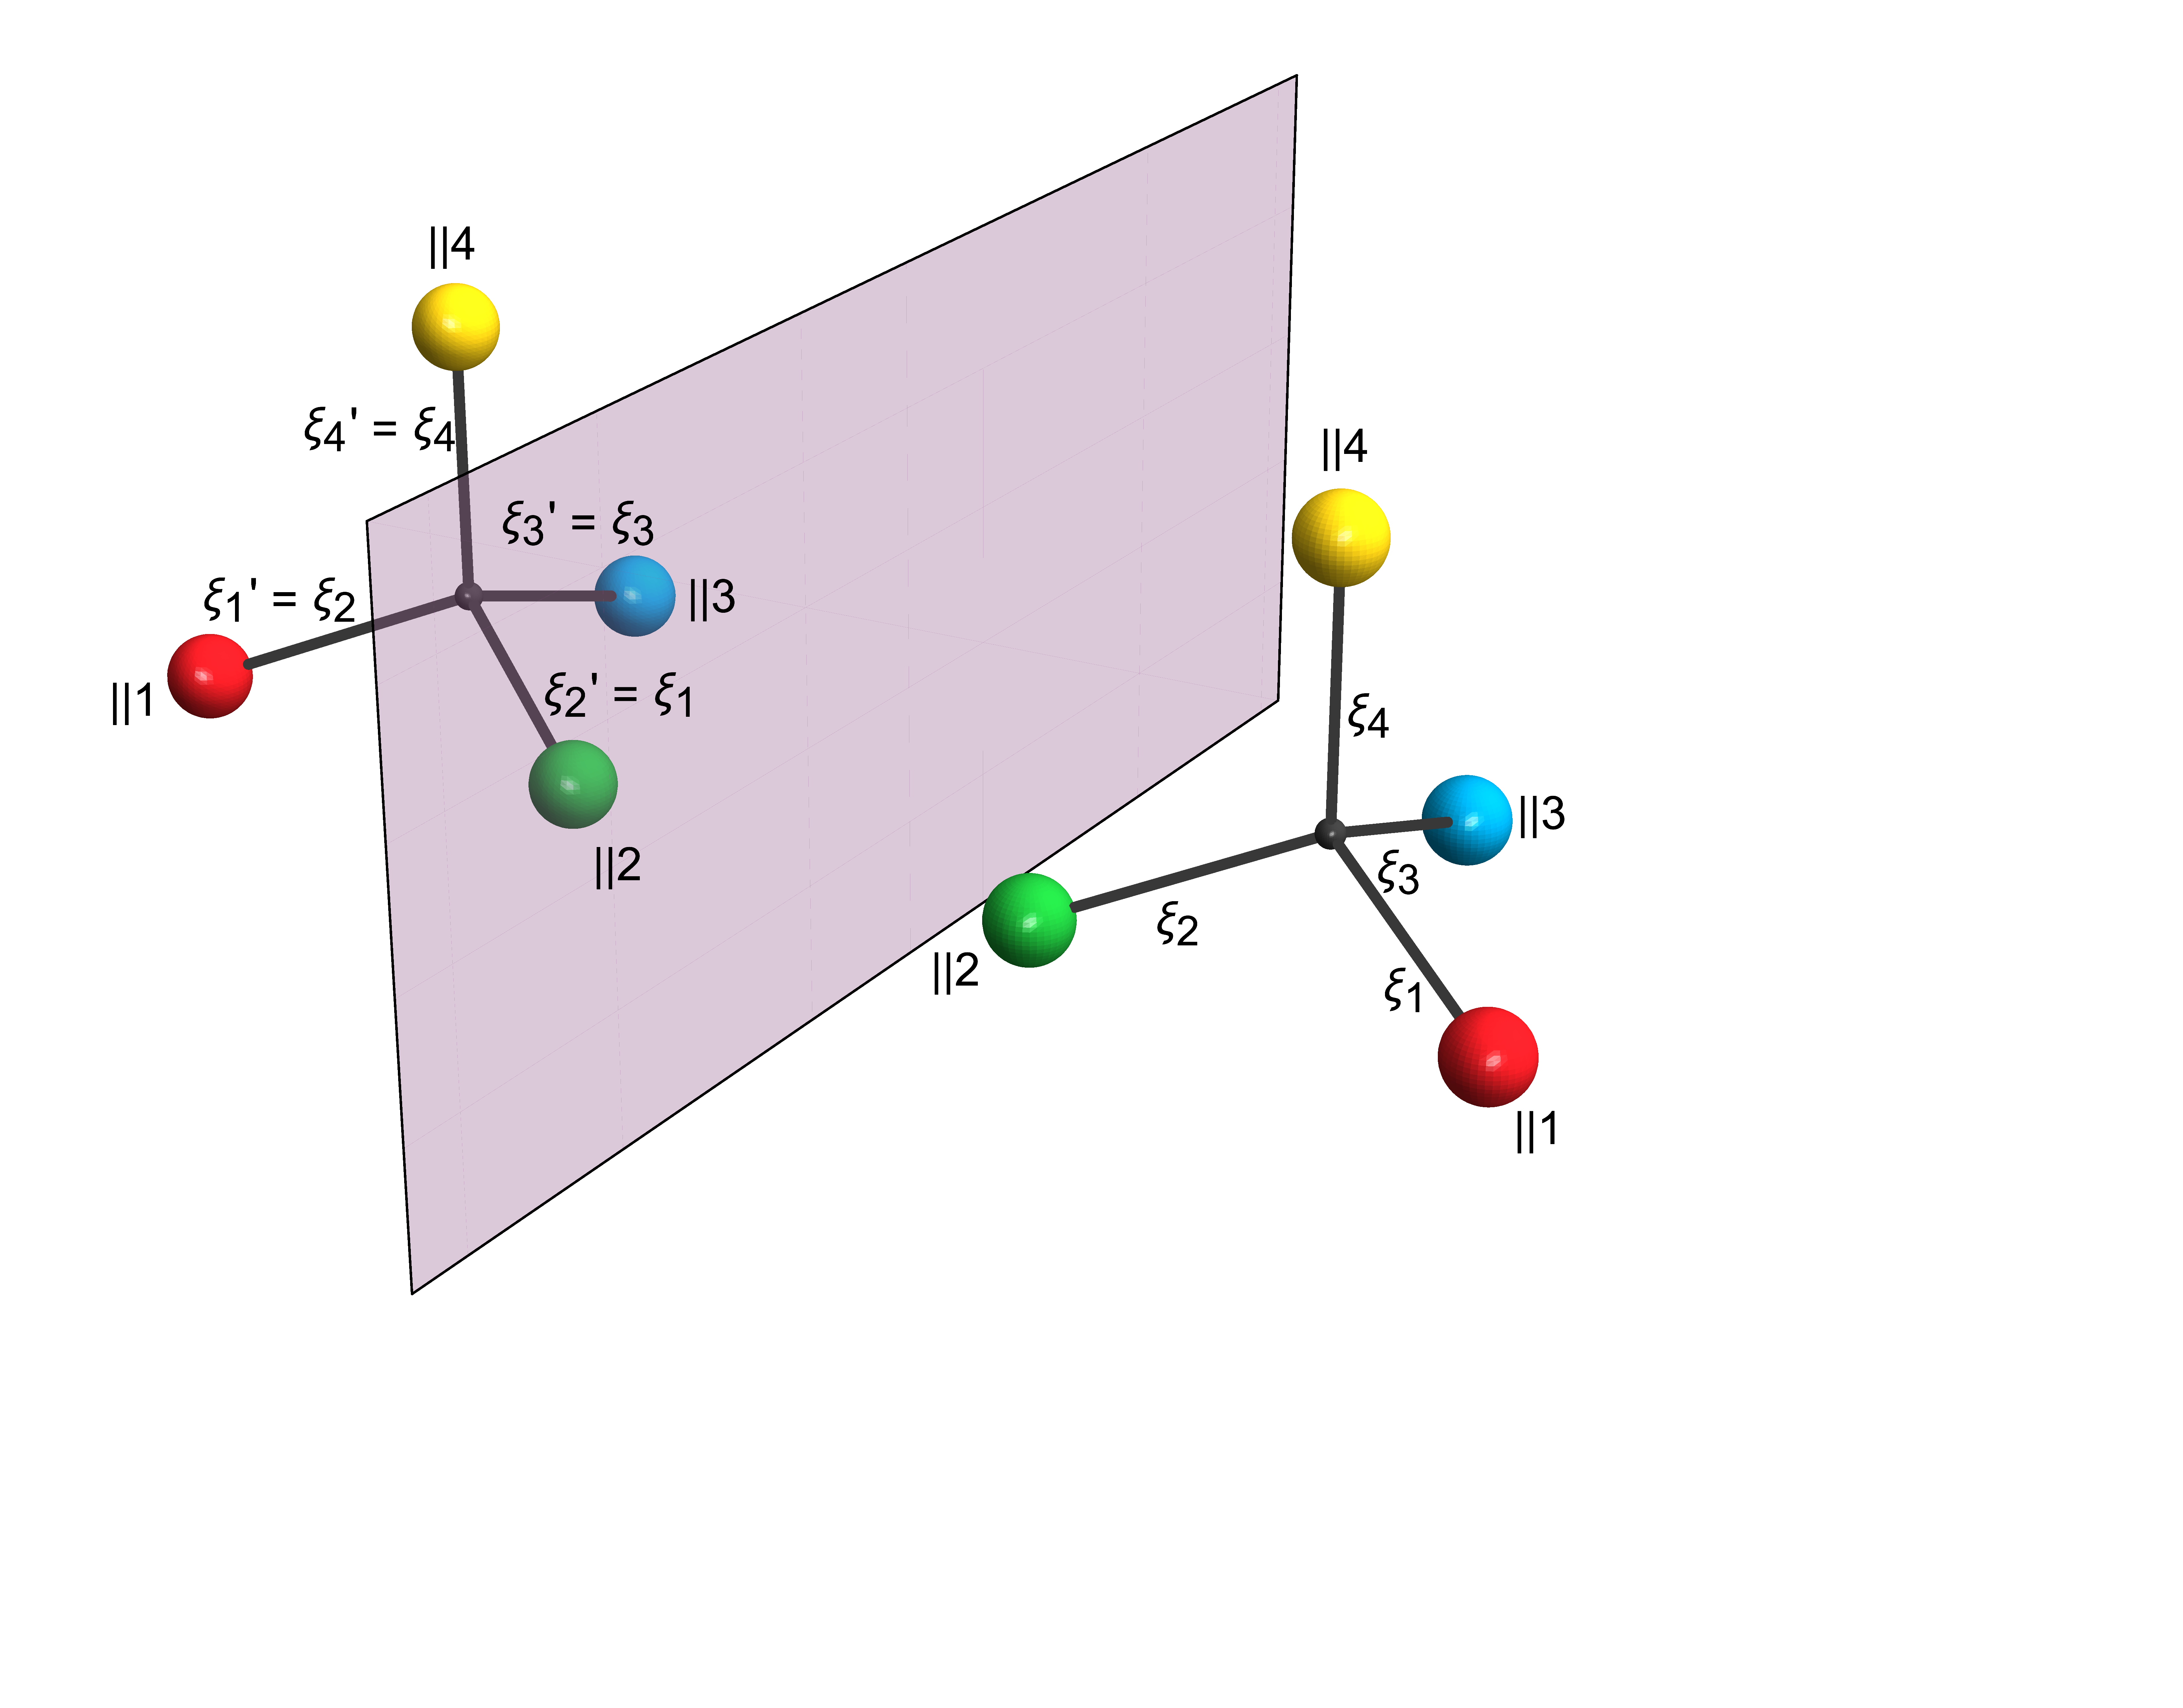
\includegraphics[width = 0.9\textwidth]{/Users/philipp/Documents/GitHub/stage_cmap/images/reflection.png}
\caption{The reflection $S_{12}$ applied to \textsc{SPr4} in the reference orientation corresponding to the swap $(||1 \leftrightsquigarrow ||2)$ }
\label{fig:reflection of swimmer}
\end{figure}

\begin{remark}
In physical terms, the previous condition stems from the invariance of Stokes equations with respect to the observation point, see figure \ref{fig:reflection of swimmer}. In fact, an observer watching the dynamics of $\gamma(S_{ij}c_0, I, \xi)$ of \textsc{SPr4} in a mirror in the reflection plane of $S_{ij}$ sees the dynamics $\gamma(c_0, I, P_{ij} \xi)$ of a micro-swimmer obtained from \textsc{SPr4} by swapping arms $||i$ and $||j$.
\end{remark}


To avoid chaos in our notation, we treat the spatial and angular parts now separately. For the spatial part, we find

\begin{proposition}
\label{prop: spatial permutation invariance}
If the control system (\ref{eq: control system}) is invariant under the swap $(||i \leftrightsquigarrow ||j)$ and $T_{\xi} \M \simeq \R^4$ for all $\xi \in \M$, then for all $\xi \in \M$
\begin{align}
	 F_c(P_{ij} \xi) = S_{ij} F_c(\xi) P_{ij}.
\end{align}
\end{proposition}

\begin{proof}
Let $\gamma_c(c_0, R_0, P_{ij} \xi)$ be the spatial part of any solution of the control problem (\ref{eq:dynamical system}). The hypothesis of rotational invariance, i.e. (\ref{eq:spatial rotational invariance}), implies that
\begin{equation}
	\gamma_c(c_0, R_0, P_{ij} \xi) = R_0 \gamma_c(c_0, I, P_{ij} \xi) + (I - R_0)c_0.
\end{equation}
From condition \ref{cond:swap}, we then get
\begin{equation}
\label{eq:spatial permutation invariance int1}
	\gamma_c(c_0, R_0, P_{ij}\xi) = R_0 S_{ij} \gamma_c(S_{ij} c_0, I, \xi) + (I - R_0)c_0.
\end{equation}
As both $\gamma_c(c_0, R_0, P_{ij} \xi)$ and $\gamma_c(S_{ij} c_0, I, \xi)$ are spatial parts of solutions of the control system (\ref{eq:dynamical system}), we have on the one hand using Proposition \ref{prop: rotational invariance}
\begin{equation}
\label{eq: spatial permutation invariance int2}
	\dot{\gamma_c}(c_0, R_0, P_{ij} \xi) = \gamma_{\theta}(c_0, R_0, P_{ij} \xi) F_c(P_{ij} \xi) P_{ij} \dot{\xi},
\end{equation}
and on the other hand using (\ref{eq:spatial permutation invariance int1}) and once more (\ref{eq:dynamical system}) together with Proposition \ref{prop: rotational invariance}
\begin{equation}
\label{eq: spatial permutation invariance int3}
	\dot{\gamma_c}(c_0, R_0, P_{ij} \xi) = R_0 S_{ij} \dot{\gamma}_c(S_{ij} c_0, I, \xi) = R_0 S_{ij} \gamma_\theta(S_{ij} c_0, I, \xi) F_c(\xi) \dot{\xi}.
\end{equation}
Equating (\ref{eq: spatial permutation invariance int2}) and (\ref{eq: spatial permutation invariance int3}) at $t = 0$ yields $ F_c(P_{ij} \xi_0) = S_{ij} F_c(\xi_0) P_{ij}$, since by hypothesis $T_{\xi_0} \M \simeq \R^4$. As $\xi_0$ was arbitrary, we conclude.
\end{proof}

%For the angular part, we first have to choose a basis and fix some notation. Naturally, we choose the canonical basis $\mathcal{E} := (e_1, e_2, e_3, e_4)$ for $\R^4$. For $\so(3)$, we choose the basis $\mathcal{L} := (L_1, L_2, L_3)$, where the matrices $L_i$ are defined in (\ref{eq: L1}) - (\ref{eq: L3}). Then we denote the matrix representing an arbitrary linear map $T: V \to W$ between two vector spaces $V$ and $W$ with respect to two bases $\mathcal{B}$ and $\mathcal{B}'$ by $[T]_{\mathcal{B}}^{\mathcal{B}'}$. Subsequently, we will especially make use of the adjoint map on $\so(3)$ associated to an orthogonal transformation $Q$ of $\R^3$. More precisely, if $Q$ is an orthogonal transformation of $\R^3$, we define the adjoint map $\ad_Q : \so(3) \to \so(3)$ by
%\begin{equation}
%\ad_Q(M) := Q M Q^T,
%\end{equation}
%which is clearly a linear map.
%
%Thus, before we address the invariance property of the angular part of the control system under a swap of arms, let us prove the following
%
%\begin{lemma}
%\label{lem:representation matrix of adjoint of reflection}
%Let $S: \R^3 \to \R^3$ be an arbitrary reflection at a plane. Then the representation matrix of the adjoint map $\ad_S$ is given by $[\ad_S]_{\mathcal{L}} = -S$.
%\end{lemma}
%
%
%\begin{proof}
%We have already seen in the proof of Lemma \ref{lem:mirror image of orientation} that for the reflection $S_i$ of the $\hat{e}_i$-axis, we have $[\ad_{S_i}]_{\mathcal{L}} = -S_i$. Moreover, by direct calculation, we find for the elementary rotations $R_i(\theta)$ that $[\ad_{R_i(\theta)}]_{\mathcal{L}} = R_{i}(\theta)$. Now if $S$ is an arbitrary reflection, we find $Q \in SO(3)$ such that $S = Q S_i Q^T$ for one of the elementary reflections $S_i$. In particular, we find by Euler's rotation theorem three angles $\alpha, \beta, \gamma \in \R$ such that $Q = R_{3}(\gamma) R_{2}(\beta) R_{1}(\alpha)$ and therefore
%\begin{equation}
%\ad_Q = \ad_{R_3(\gamma)} \circ \ad_{R_{2}(\beta)} \circ \ad_{R_{1}(\alpha)},
%\end{equation}
%which implies that $[\ad_{Q}]_{\mathcal{L}} = Q$. Since we clearly have $\ad_{Q}^{-1} = \ad_{Q^{-1}} = \ad_{Q^T}$, we have $[\ad_{Q^T}]_{\mathcal{L}} = Q^T$. Hence, due to $\ad_S = \ad_Q \circ \ad_{S_i} \circ \ad_{Q^T}$, we find
%\begin{equation}
%[\ad_S]_{\mathcal{L}} = - Q S_i Q^T = -S,
%\end{equation}
%as desired.
%\end{proof}
For the angular part, we have now the following result, in the proof of which we exploit the first, more general statement of Lemma \ref{lem:mirror image of orientation}:
\begin{proposition}
\label{prop: angular permutation invariance}
If the control system (\ref{eq:dynamical system}) is invariant under the swap $(||i \leftrightsquigarrow ||j)$ and $T_{\xi}\M \simeq \R^4$ for all $\xi \in \M$, then for all $\xi \in \M$
\begin{equation}
[F_{\theta}(P_{ij} \xi)]_{\mathcal{E}}^{\mathcal{L}} = - S_{ij} [F_{\theta}(\xi)]_{\mathcal{E}}^{\mathcal{L}} P_{ij}.
\end{equation}
\end{proposition}

\begin{proof}
Let $\gamma_\theta(c_0, R_0, P_{ij}\xi)$ be the angular part of any solution of the control problem (\ref{eq:dynamical system}). By the rotational invariance hypothesis, i.e. (\ref{eq: angular rotational invariance}), we have
\begin{equation}
	\gamma_\theta(c_0, R_0, P_{ij}\xi) = R_0 \gamma_\theta(c_0, I, \xi).
\end{equation}
Then Condition \ref{cond:swap} implies that
\begin{equation}
\label{eq: angular permutation invariance int1}
	\gamma_\theta(c_0, R_0,P_{ij} \xi) = R_0 S_{ij} \gamma_\theta(S_{ij}c_0, I, \xi) S_{ij}.
\end{equation}
Since both $\gamma_\theta(c_0, R_0, P_{ij} \xi)$ and $\gamma_\theta(S_{ij} c_0, I, \xi)$ are the angular parts of solutions of the control problem (\ref{eq:dynamical system}), we obtain with Proposition \ref{prop: rotational invariance} on the one hand
\begin{equation}
\label{eq: angular permutation invariance int2}
	\dot{\gamma_\theta}(c_0, R_0, P_{ij} \xi)= \gamma_\theta(c_0, R_0, P_{ij} \xi) F_{\theta}(P_{ij} \xi) P_{ij } \dot{\xi}
\end{equation}
and on the other hand using (\ref{eq: angular permutation invariance int1}) and once more Proposition \ref{prop: rotational invariance}
\begin{equation}
\label{eq: angular permutation invariance int3}
	\dot{\gamma_\theta}(c_0, R_0, P_{ij} \xi) =  R_0 S_{ij} \dot{\gamma_\theta}(S_{ij} c_0, I, \xi) S_{ij} = R_0 S_{ij} \gamma_\theta(S_{ij} c_0, I, \xi) F_{\theta}(\xi) \dot{\xi} S_{ij}.
\end{equation}
Imposing equality of (\ref{eq: angular permutation invariance int2}) and (\ref{eq: angular permutation invariance int3}) at $t = 0$ yields
\begin{equation}
	F_{\theta}(P_{ij} \xi_0) P_{ij}  \dot{\xi}(0) = S_{ij} F_{\theta}(\xi_0) \dot{\xi}(0) S_{ij}.
\end{equation}
By choice of the canonical basis for $\R^4$ we clearly have $[P_{ij}]_{\mathcal{E}}^{\mathcal{E}} = P_{ij}$. Therefore, by Lemma \ref{lem:mirror image of orientation}, we have
\begin{equation}
	[F_{\theta}(P_{ij} \xi_0)]_{\mathcal{E}}^{\mathcal{L}}  P_{ij} [\dot{\xi}(0)]_{\mathcal{E}} = [S_{ij} F_{\theta}(\xi_0) \dot{\xi}(0) S_{ij}]_{\mathcal{L}} = -S_{ij} [F_{\theta}(\xi_0)]_{\mathcal{E}}^{\mathcal{L}} [\dot{\xi}(0)]_{\mathcal{E}}.
\end{equation}
Recalling that $T_{\xi_0} \M \simeq \R^4$ as well as the arbitrariness of $\xi_0$ finish the proof.
\end{proof}

In the following sections, we will always understand $F_{\theta}(\xi)$ as a matrix of size $3 \times 4$ and thus, since no confusion may arise, we will abandon the slightly cumbersome notation and identify $[F_{\theta}(\xi)]_{\mathcal{E}}^{\mathcal{L}}$ with $F_{\theta}(\xi)$.





